\section{\label{II_2_A}Outils utilisés}

Si pour la tâche de segmentation automatique, nous avons écarté les architectures de modèles fondés sur des réseaux de neurones, la reconnaissance d'objets dans l'image suppose une prédiction fondée sur un apprentissage machine profond des réseaux de neurones. En effet, la plupart des outils de reconnaissance d'objets dans l'image sont fondés sur des modèles de réseaux de neurones convolutifs (CNN) dont nous avons exposé le fonctionnement dans la section précédente. Dans le domaine du patrimoine, dont le logiciel de Skinsoft gère les données des institutions, se pose la question d'une infrastructure adaptée qui permet d'assurer la sécurité des données produites. Les solutions commerciales d'analyse automatique sont pour la plupart fondées sur un Cloud externe qui implique le déplacement des données. Ces solutions sont inadaptées au contexte d'analyse de données patrimoniales en raison de propriété intellectuelle et de sécurité. Ainsi, le principe retenu afin de guider notre choix d'outil est celui d'"amener l'algorithme aux données [Traduction personnelle]" \footnote{\textit{"bring algorithms to the data"}}, via un développement local interne des modèles d'analyse \footcite{noord2021}. Afin de répondre à cette contrainte, notre choix s'est trouné vers des modèles en libre accès. Nous détaillerons dans cette section l’utilisation de l’architecture \gls{yolo}, une série d’algorithmes dédiés à la détection d’objets visuels dans les images et les flux vidéo, et fondé sur les réseaux neuronaux convolutifs, développé par Joseph Redmond en 2015, puis repris par Ultralytics en 2020 \footcite{talbi2025}. 
C’est l’un des outils de détection d’objets les plus documentés, y compris dans le domaine des sciences humaines et du patrimoine. Fondé sur la \gls{Vision par ordinateur} et entraîné grâce à des méthodes d'\gls{Apprentissage profond}, \gls{yolo} est en accès libre, et permet notamment la détection d'objets et la classification d'images, permettant ainsi de poser les bases d’une indexation \footcite{jocher2022}. Le modèle extrait dans un premier temps les caractéristiques visuelles de l'image qui lui est donnée, les agrège, afin de finalement proposer une détection d'objets \footcite{norindr2023}. Les versions récentes du modèle telles que YoLo12 ne sont désormais plus seulement basées sur des \gls{cnn} mais sur des mécanismes d'auto-attention, similaires à ceux des \gls{Transformers} dont nous avions évoqué l'architecture \footcite{2025b}. Toutefois, comme nous l'avions évoqué, cette architecture demande une consommation de mémoire élevée et une puissance de calcul lourde \footcite{2025b}. Ultralytics, créateur du modèle, recommande des versions moins avancées pour une mise en application rapide, telles que la version Yolov8, uniquement fondée sur un réseau de neurones convolutif \footcite{2023c}. Yolov8 propose une version optimisée de cette architecture en trois temps : extraction, aggrégation, et détection \footcite{yaseen2024}. Le modèle se caractérise par sa capacité à analyser l'image en une seule fois, contrairement à d'autres modèles dont les résultats impliquent plusieurs analyses de certaines parties de l'image \footcite{redmon2016}.  
Si la détection d’objets prévue par \gls{yolo} peut être appliqué à des flux vidéo, nous souhaitons l'intégrer comme composant complémentaire au processus de segmentation précédemment décrit. De fait, il être pertinent de réutiliser l'image clé fixe, produite et sauvegardée par l'outil pyscenedetect, associée à chaque séquence, afin de la faire analyser par le modèle. Ceci permettrait de réduire le temps de calcul du processus et d'améliorer l'efficacité des prédictions, puisque le modèle reçoit un minimum d’informations.  
Ainsi, l’application du modèle \gls{yolo} s’impose comme la suite logique du pipeline de segmentation détaillé précédemment, afin d’indexer les segments produits, via l’utilisation des \gls{imgcle}. Si le premier processus de segmentation produit des données temporelles associées à chaque séquence sous la forme de time codes, \gls{yolo} produit des données sémantiques sur ces mêmes séquences. À l'issue de l'analyse d'une \gls{imgcle}, le modèle \gls{yolo} est capable de produire trois types de données : des étiquettes sur les objets identifiés, un score de confiance qui indique l'indice de certitude concernant la prédiction, des coordonnées spatiales de localisation de l'objet détecté dans l'image \footcite{redmon2016}. Les étiquettes produites sur les objets identifiés, permettant de décrire les caractéristiques de l’image, pourront être indexées comme des mots-clés au sein du logiciel de gestion des collections. Le processus de détection d'objets prévu par \gls{yolo} à partir de l'image clé peut être schématisé ainsi : 

\begin{figure}[H] 
	
	\centering 
	
	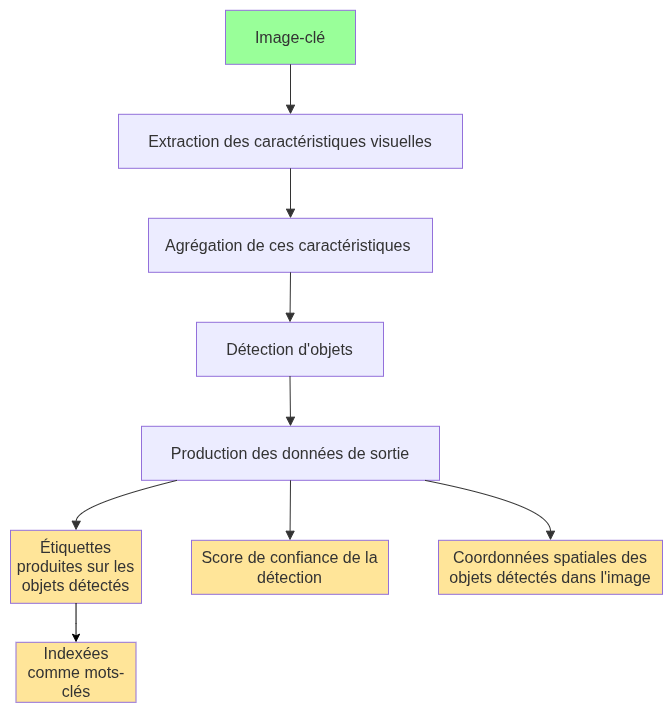
\includegraphics[width=0.7\textwidth]{images/yolo.png} 
	
	\caption{Processus de détection d'objets de \gls{yolo}} 
	
	\label{fig:yolo} 
	
\end{figure}

Les mots-clés produits à partir des étiquettes sont ensuite associés aux time-codes de chaque séquence détectée. Ainsi, chaque séquence contiendrait les données suivantes : des time codes qui l'identifient comme extrait, des étiquettes/mots-clés sur les objets qu'elle contient, et des données qui permettraient aux utilisateurs de vérifier la prédiction et de la valider. Le score de confiance produit par le modèle, permet en effet d'indiquer à l'utilisateur la certitude de l'étiquette associée à tel objet détecté. De même, les coordonnées spatiales de l’étiquette produite permettent à l’utilisateur de vérifier dans l'image si l'étiquette produite est associée au bon objet.  